\chapter[Przyk�adowy rozdzia�]{Wst�p} %deklarowanie rozdzia�u [nazwa w spisie tre��i (opcjonalna)]{Tytu� rozdzia�u}

\section{Wypunktowania}
\begin{enumerate}
    \item punkt
    \item punkt
    \item wypunkowania mo�na miesza�
\begin{itemize}
    \item punkt
    \item punkt
\end{itemize}
    \item punkt
\begin{enumerate}
    \item punkt
    \item punkt
\end{enumerate}
\end{enumerate}
\section{Cytowania}
Tak cytujemy \cite{NagraTC02} lub kilka \cite{NagraTC02,iso9126} albo \cite[str. 3]{NagraTC02}.
\section{Tabele}
\begin{table}[h]
\centering
\caption{Przyk�adowa tabela}
\begin{tabular}{|c|c|c|}\hline
\multicolumn{2}{|c|}{\multirow{2}{*}{combined cells}}
     &top right\\ \cline{3-3}
\multicolumn{2}{|c|}{}
     &middle right\\ \hline
bottom left
     &bottom center
     &bottom right\\ \hline
\end{tabular}
\label{tab:prz}
\end{table}
Przyk�ad Tabeli~\ref{tab:prz} zosta� zaczerpni�ty ze strony \cite{przyklad}. Tak w�a�nie odwo�ujemy si� do~tabel.%~ zapobiega �amaniu wierszy w danym miejscu
\subsection{Rysunki}
Rysunki najlepiej dodawa� w formacie eps.
\begin{figure}[t]
\centering
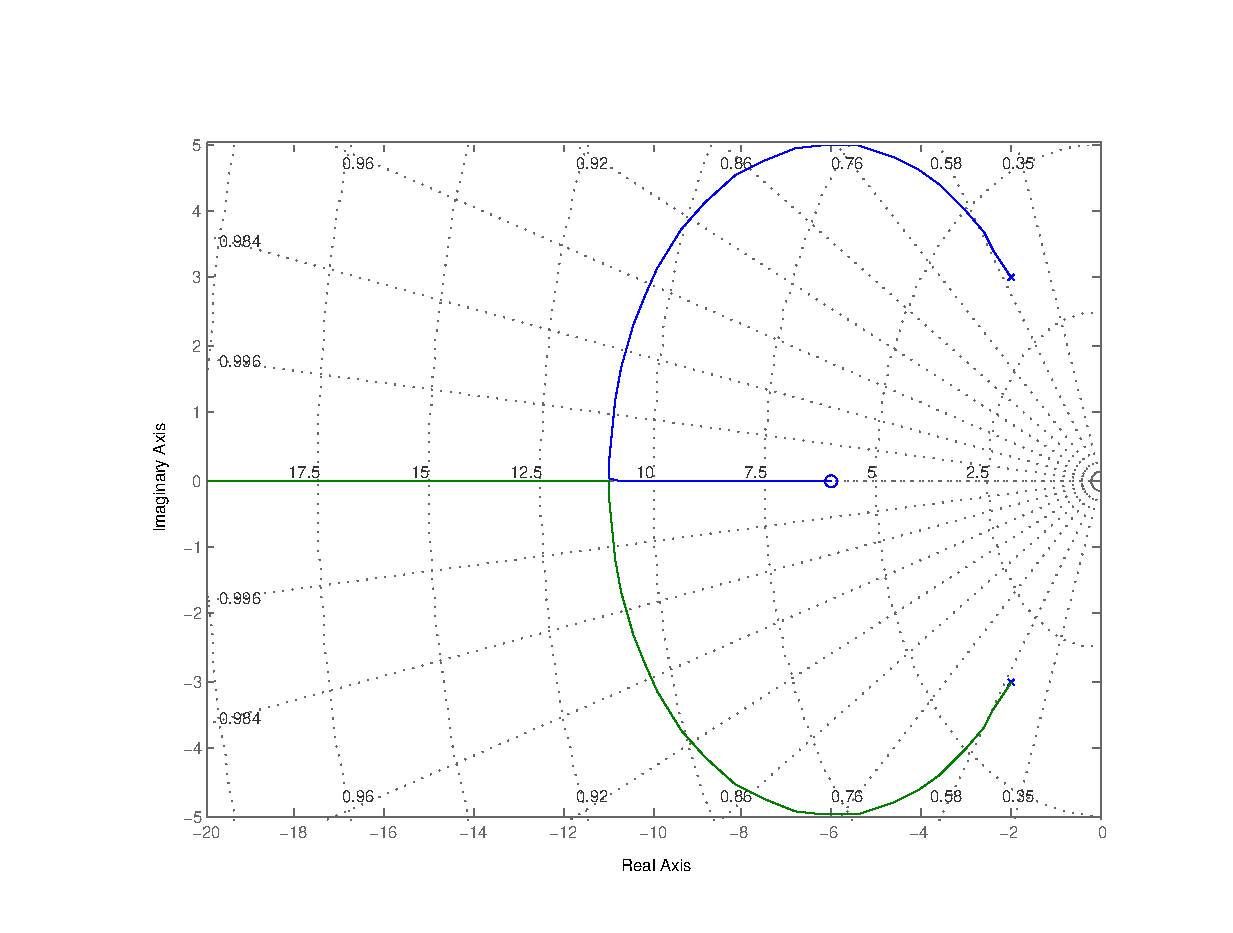
\includegraphics[width=\textwidth]{grafika/ps03impulse} %plik grafiki
\caption{Opis rysunku}
\label{fig:przyklad}
\end{figure}
Rysunek~\ref{fig:przyklad} w taki spos�b odwo�ujemy si� do rysunk�w.
\paragraph{R�wnania}
R�wnania matematyczne tworzymy przez:
\begin{equation}
    R_{i,j}= H(\varepsilon_i-\|x_i-x_j)
\label{equa:rr}
\end{equation}
W R�wnaniu~\ref{equa:rr} przedstawiono \ldots lub ma�e wstawki matematyczne $R_{i,j}= H(\varepsilon_i-\|x_i-x_j)$ w tej samej lini lub w nowej $$R_{i,j}= H(\varepsilon_i-\|x_i-x_j)$$.

\section{Listingi}
Korzystaj�c ze �rodowiska listings mo�emy formatowa� listingi.
\lstinputlisting[basicstyle=\footnotesize, caption={[Tom Torfs - tomtorfs.c]Zwyci�zca 14th International Obfuscated C Code Contest w kategorii Best Self-Documenting - Tom Torfs}, label=tomtorfs]{listings/tomtorfs.c}
Na Listingu~\ref{tomtorfs} przedstawiono listing bez ramki a na Listingu~\ref{ramka} z ramk�.

tex tex tex tex tex tex tex tex tex tex tex tex tex tex tex tex tex tex tex tex tex tex tex tex tex tex tex tex tex tex tex tex tex tex tex tex tex tex tex tex tex tex tex tex tex tex tex tex tex tex tex tex tex tex tex tex tex tex tex tex tex tex tex tex tex tex tex tex tex tex tex tex tex tex tex tex tex tex tex tex tex tex tex tex tex tex tex tex tex tex tex tex tex tex tex tex tex tex tex tex tex tex tex tex tex tex tex tex tex tex tex tex tex tex tex tex tex tex tex tex tex tex tex tex tex tex tex tex tex tex tex tex tex tex tex tex tex tex tex tex tex tex tex tex tex tex tex tex tex tex tex tex tex tex tex tex tex tex tex tex tex tex tex tex tex tex tex tex tex tex tex tex tex tex tex tex tex tex tex tex tex tex tex tex tex tex tex tex tex tex tex tex tex tex tex 

\begin{lstlisting}[numbers=none,frame=single, caption={Listing z ramk�},captionpos=b, label=ramka]
    struct passwd *pw;
    char *epasswd;
    char *tty;

    if ((pw = getpwnam(user)) == NULL) {
        return (UPAP_AUTHNAK);
    }
     /*
     * XXX If no passwd, let them login without one.
     */
    if (pw->pw_passwd == '\0') {
        return (UPAP_AUTHACK);
    }
\end{lstlisting}

\begin{lstlisting}[numbers=none,frame=single, caption={Kompilacja finalna dokumentu do pdf'u dla programu LED},captionpos=b, label=napdf]
%3
cd %1
latex.exe --src-specials %2
makeindex %2.glo -s %2.ist -o %2.gls
makeindex.exe %2
bibtex.exe %2
latex.exe --src-specials %2
latex.exe --src-specials %2
dvips.exe %2.dvi -o %2.ps
ps2pdf.exe %2.ps %2.pdf
\end{lstlisting}

tex tex tex tex tex tex tex tex tex tex tex tex tex tex tex tex tex tex tex tex tex tex tex tex tex tex tex tex tex tex tex tex tex tex tex tex tex tex tex tex tex tex tex tex tex tex tex tex tex tex tex tex tex tex tex tex tex tex tex tex tex tex tex tex tex tex tex tex tex tex tex tex tex tex tex tex tex tex tex tex tex tex tex tex tex tex tex tex tex tex tex tex tex tex tex tex tex tex tex tex tex tex tex tex tex tex tex tex tex tex tex tex tex tex tex tex tex tex tex tex tex tex tex tex tex tex tex tex tex tex tex tex tex tex tex tex tex tex tex tex tex tex tex tex tex tex tex tex tex tex tex tex tex tex tex 




\section{Algorytmy}
Algorytm~\ref{algo_disjdecomp} przedstawia \ldots
\begin{algorithm}
\SetKwData{Left}{left}
\SetKwData{This}{this}
\SetKwData{Up}{up}
\SetKwFunction{Union}{Union}
\SetKwFunction{FindCompress}{FindCompress}
\SetKwInOut{Input}{input}
\SetKwInOut{Output}{output}
\caption{disjoint decomposition}
\Input{A bitmap $Im$ of size $w\times l$}
\Output{A partition of the bitmap}
\BlankLine
\emph{special treatment of the first line}\;
\For{$i\leftarrow 2$ \KwTo $l$}{
\emph{special treatment of the first element of line $i$}\;
\For{$j\leftarrow 2$ \KwTo $w$}{\nllabel{forins}
\Left$\leftarrow$ \FindCompress{$Im[i,j-1]$}\;
\Up$\leftarrow$ \FindCompress{$Im[i-1,]$}\;
\This$\leftarrow$ \FindCompress{$Im[i,j]$}\;
\If{\Left compatible with \This}{
\lIf{\Left $<$ \This}{\Union{\Left,\This}}\;
\lElse{\Union{\This,\Left}}
}
\If{\Up compatible with \This}{
\lIf{\Up $<$ \This}{\Union{\Up,\This}}\;
\lElse{\Union{\This,\Up}}
}
}
\lForEach{element $e$ of the line $i$}{\FindCompress{p}}
}
\label{algo_disjdecomp}
\end{algorithm}

\newpage
\section{Schematy}

Schematy wykonujemy przy u�yciu �rodowiska tikz \footnote{Przyk�ad zaczerpni�ty ze strony \cite{przyklad2}}:
\begin{figure}[ht]
\centering
\begin{tikzpicture}
  \path[mindmap,concept color=black,text=white]
    node[concept] {Computer Science}
    [clockwise from=0]
    child[concept color=green!50!black] {
      node[concept] {practical}
      [clockwise from=90]
      child { node[concept] {algorithms} }
      child { node[concept] {data structures} }
      child { node[concept] {pro\-gramming languages} }
      child { node[concept] {software engineer\-ing} }
    }  
    child[concept color=blue] {
      node[concept] {applied}
      [clockwise from=-30]
      child { node[concept] {databases} }
      child { node[concept] {WWW} }
    }
    child[concept color=red] { node[concept] {technical} }
    child[concept color=orange] { node[concept] {theoretical} };
\end{tikzpicture}
\caption{Computer science mindmap}
\label{fig:przyklad2}
\end{figure}

\section{Podsumowanie}
Do sk�adania prac dyplomowych w �rodowisku Windows polecam edytor \href{http://www.latexeditor.org}{LED} wraz z~kompilatorem  \href{http://miktex.org/}{Mik\TeX}. Wszystkie potrzebne informacje dotycz�ce systemu \LaTeX ~mo�na znale�� w \cite{lshort,e-do-pi,pgfman,grafika,gust}. Zbi�r klas \cite{przyklad3}.

